% Figure reproduced from Ren et al. (2026), "Automated data synthesis and
% retrieval-augmented generation for legal large language models" (Knowledge-Based
% Systems), Fig. 2, for scholarly discussion and critique within this review. Copyright
% remains with the original authors/publisher.
\begin{figure*}[t]
\centering
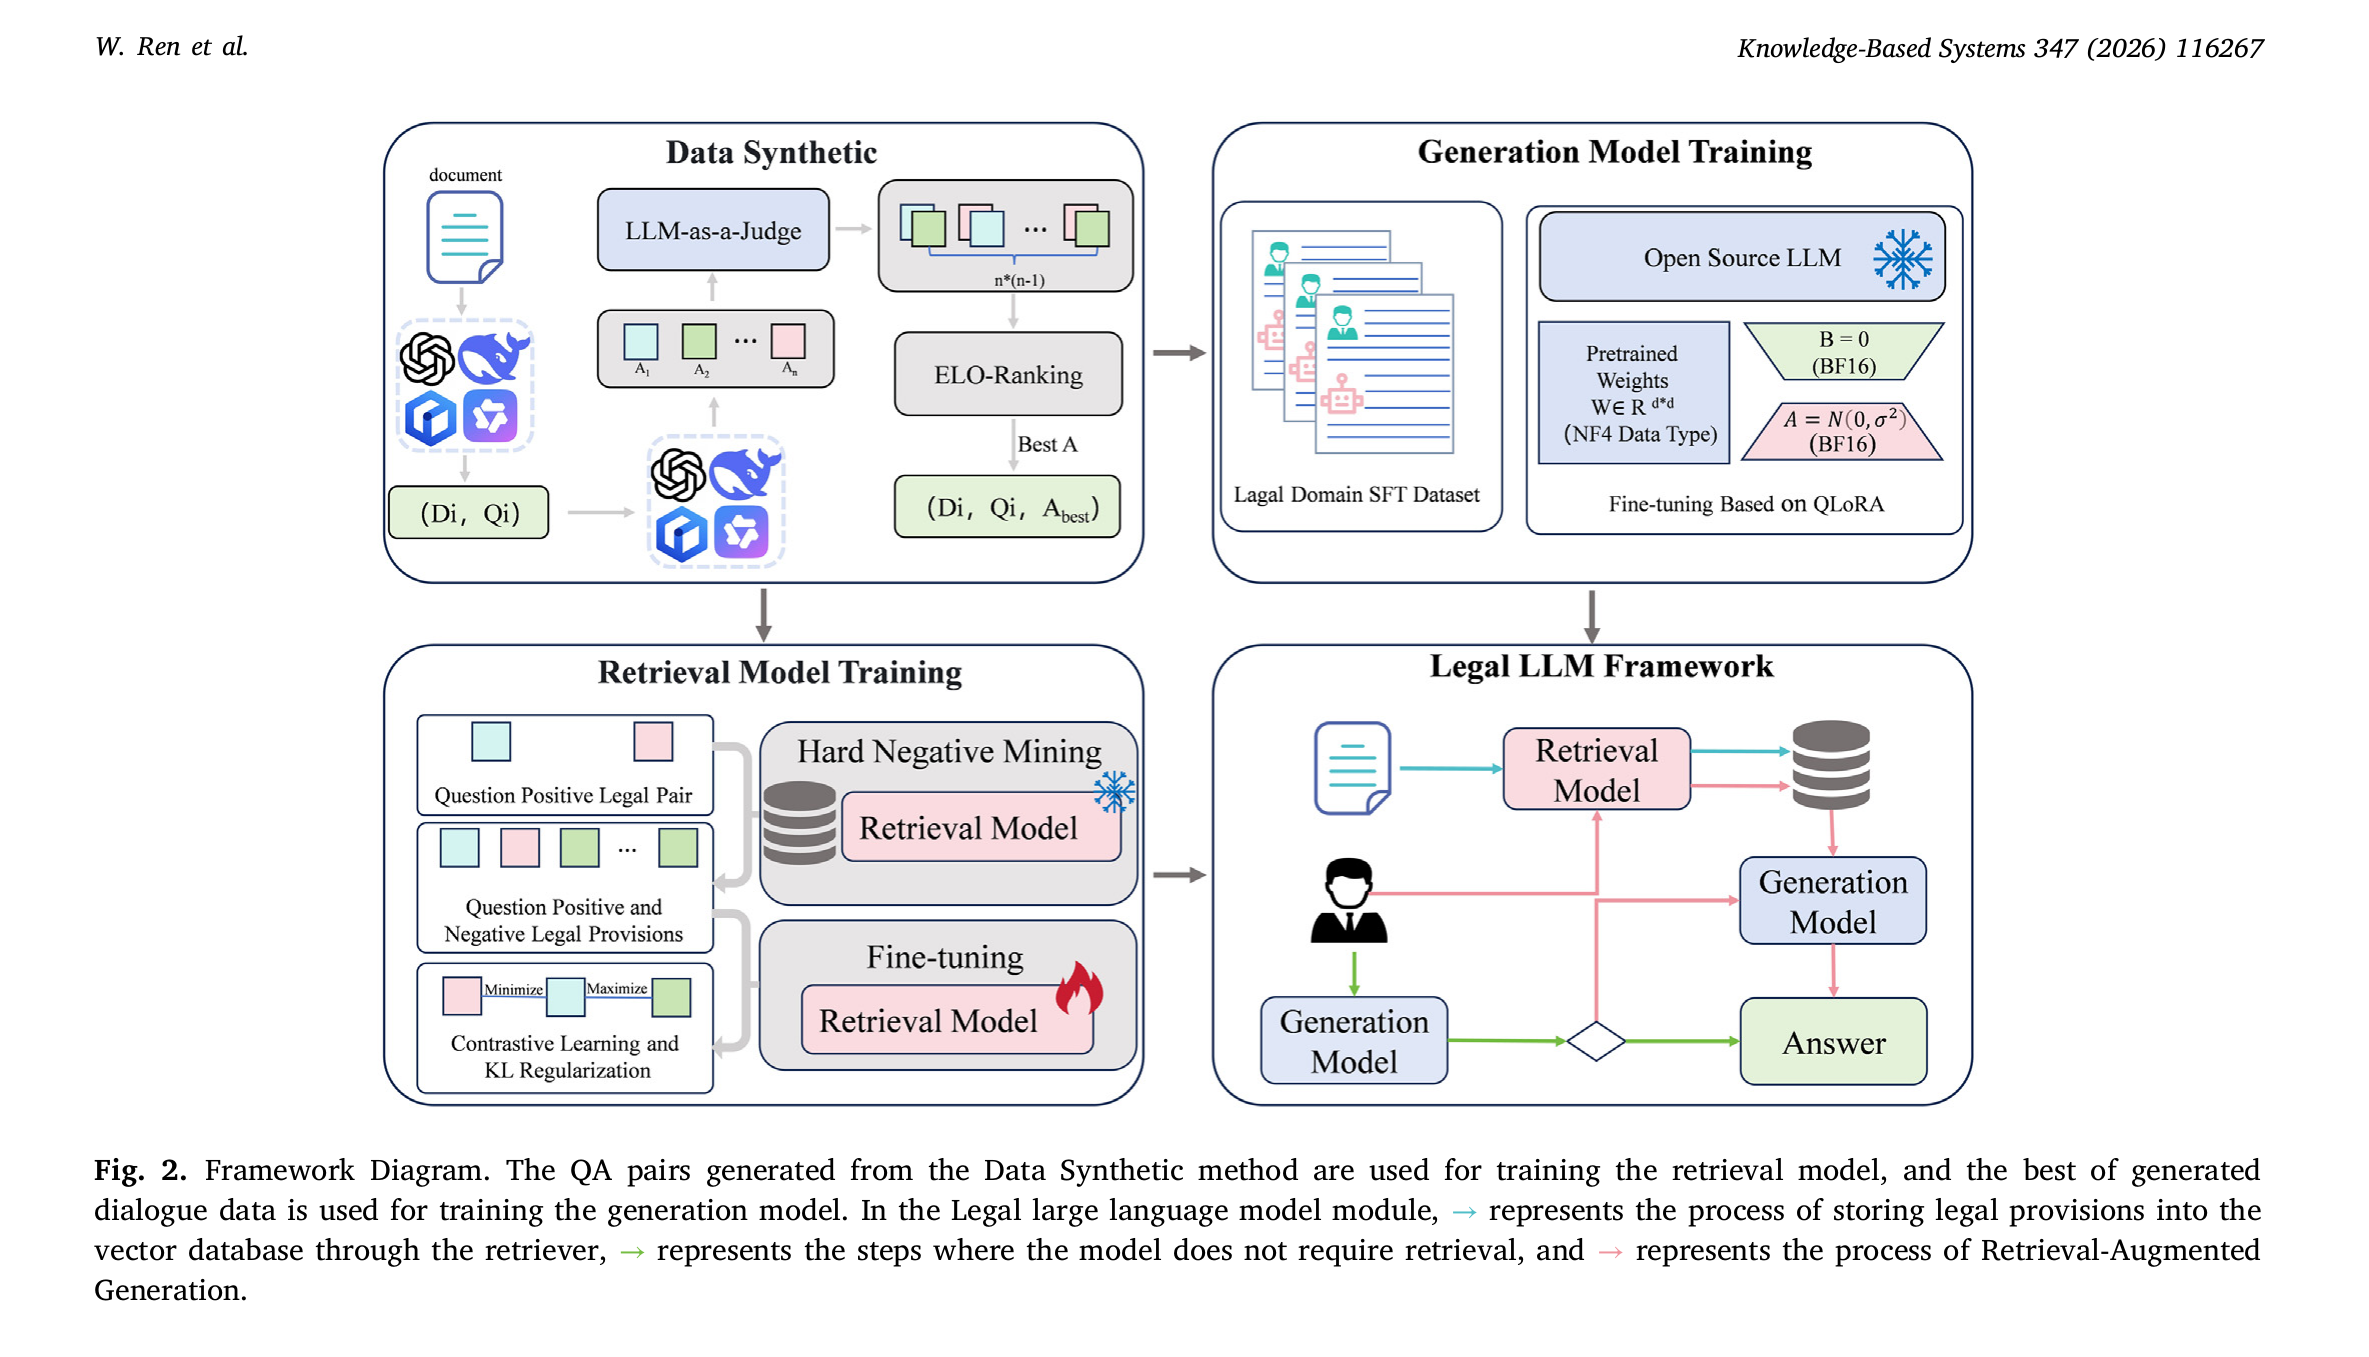
\includegraphics[width=\textwidth]{images/ren2026_fig2.png}
\caption{Figure reproduced from \citet{ren2026}: their framework diagram. QA pairs generated by
the Data Synthetic module (LLM-as-a-Judge selecting the best candidate answer via Elo-ranking)
train both the retrieval model, through hard-negative mining and contrastive fine-tuning, and the
generation model, through QLoRA fine-tuning of an open-source LLM on a legal-domain SFT dataset.
The resulting Legal LLM Framework routes a user's query through the fine-tuned retrieval model
and generation model to produce an answer, illustrating the training-data-centric design this
survey contrasts with Legalyze's evidence-centric design in Figure~\ref{fig:legalyze-ren}.}
\label{fig:ren2026-arch}
\end{figure*}
